\section{Large-Scale Bursts}
  In this section we analyze large-scale bursts in the cross traffic. We model 
  the cross traffic using a simple on-off model. The sending rate of the cross 
  traffic as a function of time is shown in Figure \ref{cross-traffic}. 
  $T_{on}$ is the duration of time while the cross traffic is sending data 
  while $T_{off}$ is the duration of time while the cross traffic is not 
  sending any data. $Ron$ is the rate at which the cross traffic is sending 
  data during $T_{on}$ and $C$ is the transmission capacity of the bottleneck 
  link.
  \begin{figure}[htb]
    \centering
    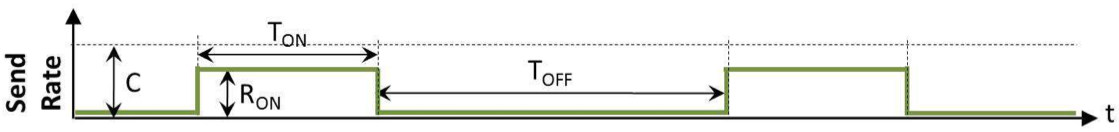
\includegraphics[width=0.9\textwidth]{img/cross-traffic.png}
    \caption{The on-off cross traffic model}
    \label{cross-traffic}
  \end{figure}

  We define large-scale bursts as on-off cross traffic were Rapid has 
  enough time to adapt its sending rate to the available bandwidth. Figure 
  \ref{large-burst} shows the interaction between Rapid throughput and a 
  large-scale burst on-off cross traffic, where $D$ is the queue drain time.
  \begin{figure}[htb]
    \centering
    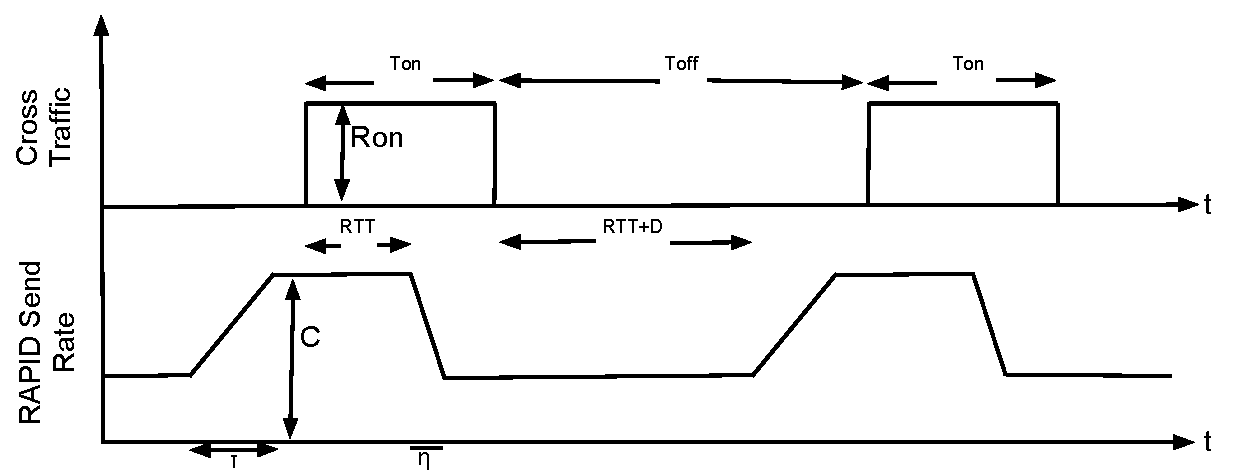
\includegraphics[width=0.9\textwidth]{img/large-burst.pdf}
    \caption{Rapid send rate and on-off cross traffic interaction}
    \label{large-burst}
  \end{figure}
  
  A large-scale burst occurs when the following inequalities are true.
  \begin{IEEEeqnarray}{rCl}
    T_{on} + D & \ge & \eta \IEEEyessubnumber
    \label{enough-to-decrease} \\
    T_{off} - D & \ge & \tau \IEEEyessubnumber
    \label{enough-to-increase}
  \end{IEEEeqnarray}
  Inequality \eqref{enough-to-decrease} is true when Rapid has enough time 
  to decrease its sending rate to $C - R_{on}$. On the other hand, inequality 
  \eqref{enough-to-increase} is true when Rapid has enough time to increase 
  its sending rate to $C$.

  Since the Rapid send rate is periodic in steady state, we can find an 
  expression for the Rapid throughput by time averaging over a period of 
  duration $T_{on} + T_{off}$. We get the following expression.
  \begin{equation}
    R = C - R_{avg} \frac{2 T_{on} + 2 D + \tau - \eta}{2 T_{on}}
    \label{r-large}
  \end{equation}
  where $R_{avg}$ is the average sending rate of the cross traffic:
  \begin{equation}
    R_{avg} = \frac{R_{on} T_{on}}{T_{on} + T_{off}}
    \label{ravg}
  \end{equation}

  Figure \ref{large-burst} shows one of the 16 different cases of large-scale 
  bursts. To find these 16 large-scale cases, we have tried different sizes 
  of $RTT$, $\tau$, and $\eta$ with respect to the sizes of $T_{on}$ and 
  $T_{off}$. We have made sure that these 16 cases are mutually exclusive. 
  However, we are not sure if these cases are exhaustive. In addition to the 
  large-scale inequalities \ref{enough-to-decrease} 
  and \ref{enough-to-increase}, the following inequalities also need to be true 
  for the particular case shown in Figure \ref{large-burst} to occur.
  \begin{IEEEeqnarray*}{rCl}
    RTT & < & T_{on} - \eta \\
    RTT & < & T_{off} - D - \tau
  \end{IEEEeqnarray*}
  For the case shown in Figure \ref{large-burst}, the queue that accumulates 
  at the bottleneck link when the sending rate of both Rapid and the cross 
  traffic exceed the bottleneck capacity is given by equation 
  \eqref{queue1}.
  \begin{equation}
    Q = R_{on} RTT + \frac{\eta R_{on}}{2}
    \label{queue1}
  \end{equation}
  Thus, the queue drain time can be expressed as
  \begin{equation}
    D = \frac{Q}{C} = \frac{R_{on} RTT}{C} + \frac{\eta R_{on}}{2C}
    \label{delay}
  \end{equation}
  Replacing equation \eqref{delay} into equation \eqref{r-large}, we get an 
  expression for the Rapid throughput $R$ as a function of $T_{on}$, 
  $T_{off}$, $R_{on}$, $C$, $\tau$, $\eta$, and $RTT$.
